\documentclass{beamer}
\usetheme{Madrid}

\usepackage{pgfplots}

\usepackage{bm}

\usepackage{color}

\usepackage{graphicx}

\title{Igeta, Takahashi, and Matsui (2018)}
\subtitle{STAT 778 Project}
\author{Tom Wallace}
\institute{George Mason University}
\date{Spring 2018}

\AtBeginSection[]{
	\begin{frame}
		\frametitle{Table of Contents}
		\tableofcontents[currentsection]
	\end{frame}
}
\begin{document}

\frame{\titlepage}

%%%%%%%%%%%%% Introduction %%%%%%%%%%%%%%

\section{Background}
\begin{frame}
	\frametitle{What is overdispersion?}
	Occurs when a dataset exhibits higher variance than expected under the assumed
	distribution \\~\\

	     Commonly occurs with \textbf{count data} \\~\\

	     Motivating example: Poisson 
	     \begin{itemize}
		     \item \small Mean = $\lambda$
		     \item \small Var = $\lambda$
		     \item \small Cannot change $\lambda$ to correct for variance without skewing
			     mean
	     \end{itemize}
\end{frame}
\begin{frame}
	\frametitle{What are the consequences of overdispersion?}
	If not corrected, overdispersion results in distorted test statistics and estimated
	standard errors \\~\\

	Practical consequences can be severe: count data is common in clinical
	trials
	\begin{itemize}
		\item \small E.g., anti-epilepsy drug might use \textit{number
			of seizures over study period} as measure of drug
			efficacy 
		\item \small Failure to correct for overdispersion could cause
			Type II error (failure to adopt beneficial treatment)
			or, even worse, Type I error (adopt treatment that is
			not beneficial and may even be harmful)
	\end{itemize}
\end{frame}
\begin{frame}
	\frametitle{How can we correct for overdispersion?}
	 Correct root cause of overdispersion if possible (e.g.,
	zero-inflated models) \\~\\

	Use count distribution that allows adjustment of variance
	independent from mean (e.g., negative binomial) \\~\\

	Approach of authors:
	\begin{itemize}
		\item \small Want to estimate treatment effect in Poisson model
			$\lambda_i = \exp{(\beta_0 + \beta_1 X_{ij})}$, but data
			is over-dispersed
		\item \small Distinguish between \textit{true} variance function
			$V$ (unknown) and \textit{working} variance
			function $\tilde{V}$
		\item \small Chances are low that we guess perfectly such that
			$V=\tilde{V}$ 
			\\~\\
	\end{itemize}

	\begin{block}{Goal of paper}
		Test statistics, power, and sample size
		calculations that are robust to misspecification of the
		variance function ($V\neq \tilde{V}$)
	\end{block}
\end{frame}
	     \section{Methods}
\begin{frame}
	\frametitle{Original contributions}
	\begin{block}{Test statistic}
		$$
		Z = \frac{\hat{\beta}_1}{\sqrt{n^{-1} \hat{W}_0}}
		$$
	\end{block}
	\begin{block}{Power of test using that statistic}
		$$
		\mathrm{Pr} \left( Z > z_{1 - \alpha/ 2} \right) 
		=
		1 - \Phi 
		\left(
		z_{1 - \alpha / 2}
		\sqrt{\frac{W_0}{W_1}}
		-
		\sqrt{n}
		\frac{\beta_1}{\sqrt{W_1}}
		\right)
		$$
	\end{block}
	\begin{block}{Sample size required to achieve desired power}
		$$
		n \geq \frac{(z_{1 - \alpha / 2} \sqrt{W_0} + z_{1 - \beta}
		\sqrt{W_1})^2}{\left( \log (\lambda_2 / \lambda_1 ) \right)^2}
		$$
	\end{block}		
\end{frame}
\begin{frame}
	\frametitle{How to use them to determine sample size}
	Authors propose the following procedure
	\begin{enumerate} 
		\item \small Consider multiple true variance functions, pick
			most plausible (how?)
		\item \small Specify working variance function
		\item \small Conduct sensitivity analysis of power under
			different misspecifications
		\item \small Adopt sample size achieving desired power
	\end{enumerate}
\end{frame}
	     \section{Implementation in C}
	     \begin{frame}
		     \frametitle{How I felt reading and trying to replicate this
		     paper}
	\begin{center}
		
\includegraphics[height=3in, keepaspectratio]{dog.jpg}
	\end{center}

	     \end{frame}
	     \begin{frame}
		     \frametitle{My progress}
		     Unable to replicate paper \\~\\

		     Primary fault lies with my own limitations
		     \begin{itemize}
			     \item \small Paper assumes that
				     readers are familiar are with many things
				     not actually covered in paper
			     \item \small This probably is a fair assumption for a
				     peer-reviewed article, but I was
				     out of my depth \\~\\
		     \end{itemize}

		    That said$\ldots$ this was a poorly written paper 
		     \begin{itemize}
			     \item \small Complex and inconsistently applied
				     notation (e.g., $\hat{\tilde{\phi}}^{*}_{p}$)
			     \item \small Apparent errors
			     \item \small Confusing presentation\\~\\
		     \end{itemize}

		     I will briefly cover some stumbling blocks
	     \end{frame}
	     \begin{frame}
		     \frametitle{Simultaneous estimation}
		     To calculate $Z$, we need to estimate
		     $\hat{\tilde{\phi}}^{*}_{p}$, the estimated dispersion
		     parameter of the working variance function under the null
		     hypothesis \\~\\

		     To estimate $\hat{\tilde{\phi}}^{*}_{p}$, we need
		     $\hat{\beta_0}^*$, the estimated ``base rate'' parameter under the
		     null hypothesis \\~\\

		     To estimate $\hat{\beta_0}^*$, we need
		     $\hat{\tilde{\phi}}^{*}_{p}$ \\~\\

		     Summary: we need A to calculate B, and B to calculate A
		     \\~\\

		     Solution: simultaneous numerical estimation of both, which
		     apparently is a common approach in GEE
	     \end{frame}
	     \begin{frame}
		     \frametitle{Estimation of treatment effect} 
		     We need to estimate $\hat{\beta}_1$ via quasi maximum
		     likelihood (QML) \\~\\ 
		     $$
	\sum_{i=1}^2 \sum_{j=1}^{n_i} \bm{D}'_{ij} \tilde{V}_{ij}^{-1}(Y_{ij}-\mu_{ij})
	= \bm{0}
		     $$ \\~\\

		     $\tilde{V}$ takes $\hat{\tilde{\phi}}^{*}_{p}$ as a
		     parameter, which I failed to find (per previous slide)
		     \\~\\

		     I identified a working variance function
		     $\tilde{V}$ for which $\hat{\tilde{\phi}}^{*}_{p}$ is
		     irrelevant in our QML equations \\~\\

		     Used Newton-Raphson to estimate, but failed to converge
		     (singular matrix) \\~\\

		     Unclear whether error is in my math or in my coding
	     \end{frame}
	     \section{Simulation Study}
	     \begin{frame}
		     \frametitle{Could not actually conduct study, but path is
		     clear}
		     Simulation study
		     \begin{enumerate}
			     \item \small Assume some true variance
				     function and some true treatment effect
				     ($\exp{(\beta_1)}$) 
			     \item \small Use authors' methods to calculate
				     required sample size 
			     \item \small Generate simulated data for control
				     and treatment group 
			     \item \small Conduct test of difference between
				     groups using authors' $Z$-statistic and
				     some assumed working variance function 
			     \item \small Record whether Type I or Type II error
				     occurred
			     \item \small Repeat many times, calculate empirical
				     Type I and Type II error rate \\~\\
		     \end{enumerate}

		     If we do this for many cases in which $V \neq \tilde{V}$,
		     and the empirical results match our theoretical
		     expectations, we conclude that the authors' claims of
		     robustness to misspecification of variance are supported
	     \end{frame}
	     \begin{frame}
		     \frametitle{Authors' results}
	\begin{center}
		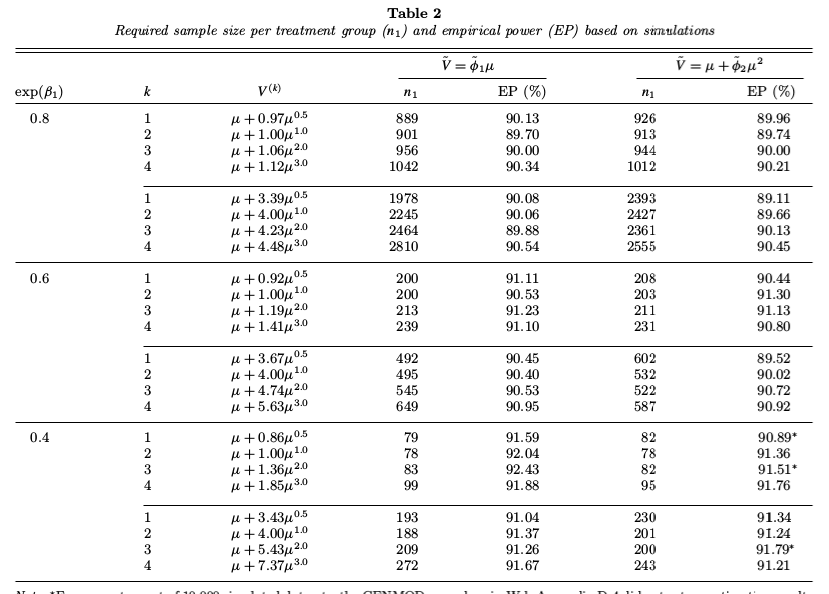
\includegraphics[height=3in, keepaspectratio]{table2.png}
	\end{center}
	     \end{frame}
	     \section{Conclusion}
	     \begin{frame}
		     \frametitle{An educational experience}
		     This paper clearly is intended to be practical and useful
		     \\~\\

		     But, poor quality of presentation means the target
		     audience (working statisticians) will ignore it---too much
		     effort to decipher, too little time \\~\\

		     It doesn't have to be this way---many of the most-cited
		     statistics papers ever are easy to read (e.g. Efron
		     1979)
		     \begin{itemize}
			     \item \small This is part of why they're so highly
				     cited!\\~\\
		     \end{itemize}

		     There is an important lesson here: \textbf{effective
		     communication of your methods is just as important as
		     formal correctness}
	     \end{frame}
\end{document}
